
\documentclass[a4paper,12pt,twoside]{report}
\usepackage[left=2cm,right=2cm,top=2cm,bottom=3cm]{geometry}


\usepackage{graphicx}
\usepackage{verbatim}
\usepackage{latexsym}
\usepackage{mathchars}
\usepackage{setspace}
\usepackage{hyperref}
\usepackage{subfigure}
\usepackage{caption}


\hypersetup{
    colorlinks=false,
    pdfborder={0 0 0},
}

\setlength{\parskip}{\medskipamount}  % a little space before a \par
\setlength{\parindent}{0pt}	      % don't indent first lines of paragraphs

%UHEAD.STY  If this is included after \documentstyle{report}, it adds
% an underlined heading style to the LaTeX report style.
% \pagestyle{uheadings} will put underlined headings at the top
% of each page. The right page headings are the Chapter titles and
% the left page titles are supplied by \def\lefthead{text}.

% Ted Shapin, Dec. 17, 1986

\makeatletter
\def\chapapp2{Chapter}

\def\appendix{\par
 \setcounter{chapter}{0}
 \setcounter{section}{0}
 \def\chapapp2{Appendix}
 \def\@chapapp{Appendix}
 \def\thechapter{\Alph{chapter}}}

\def\ps@uheadings{\let\@mkboth\markboth
% modifications
\def\@oddhead{\protect\underline{\protect\makebox[\textwidth][l]
		{\sl\rightmark\hfill\rm\thepage}}}
\def\@oddfoot{}
\def\@evenfoot{}
\def\@evenhead{\protect\underline{\protect\makebox[\textwidth][l]
		{\rm\thepage\hfill\sl\leftmark}}}
% end of modifications
\def\chaptermark##1{\markboth {\ifnum \c@secnumdepth >\m@ne
 \chapapp2\ \thechapter. \ \fi ##1}{}}%
\def\sectionmark##1{\markright {\ifnum \c@secnumdepth >\z@
   \thesection. \ \fi ##1}}}
\makeatother



%%From: marcel@cs.caltech.edu (Marcel van der Goot)
%%Newsgroups: comp.text.tex
%%Subject: illegal modification of boxit.sty
%%Date: 28 Feb 92 01:10:02 GMT
%%Organization: California Institute of Technology (CS dept)
%%Nntp-Posting-Host: andromeda.cs.caltech.edu
%%
%%
%%Quite some time ago I posted a file boxit.sty; maybe it made it
%%to some archives, although I don't recall submitting it. It defines
%%	\begin{boxit}
%%	...
%%	\end{boxit}
%%to draw a box around `...', where the `...' can contain other
%%environments (e.g., a verbatim environment). Unfortunately, it had
%%a problem: it did not work if you used it in paragraph mode, i.e., it
%%only worked if there was an empty line in front of \begin{boxit}.
%%Luckily, that is easily corrected.
%%
%%HOWEVER, apparently someone noticed the problem, tried to correct it,
%%and then distributed this modified version. That would be fine with me,
%%except that:
%%1. There was no note in the file about this modification, it only has my
%%   name in it.
%%2. The modification is wrong: now it only works if there is *no* empty
%%   line in front of \begin{boxit}. In my opinion this bug is worse than
%%   the original one.
%%
%%In particular, the author of this modification tried to force an empty
%%line by inserting a `\\' in the definition of \Beginboxit. If you have
%%a version of boxit.sty with a `\\', please delete it. If you have my
%%old version of boxit.sty, please also delete it. Below is an improved
%%version.
%%
%%Thanks to Joe Armstrong for drawing my attention to the bug and to the
%%illegal version.
%%
%%                                          Marcel van der Goot
%% .---------------------------------------------------------------
%% | Blauw de viooltjes,                    marcel@cs.caltech.edu
%% |    Rood zijn de rozen;
%% | Een rijm kan gezet
%% |    Met plaksel en dozen.
%% |


% boxit.sty
% version: 27 Feb 1992
%
% Defines a boxit environment, which draws lines around its contents.
% Usage:
%   \begin{boxit}
%	... (text you want to be boxed, can contain other environments)
%   \end{boxit}
%
% The width of the box is the width of the contents.
% The boxit* environment behaves the same, except that the box will be
% at least as wide as a normal paragraph.
%
% The reason for writing it this way (rather than with the \boxit#1 macro
% from the TeXbook), is that now you can box verbatim text, as in
%   \begin{boxit}
%   \begin{verbatim}
%   this better come out in boxed verbatim mode ...
%   \end{verbatim}
%   \end{boxit}
%
%						Marcel van der Goot
%						marcel@cs.caltech.edu
%

\def\Beginboxit
   {\par
    \vbox\bgroup
	   \hrule
	   \hbox\bgroup
		  \vrule \kern1.2pt %
		  \vbox\bgroup\kern1.2pt
   }

\def\Endboxit{%
			      \kern1.2pt
		       \egroup
		  \kern1.2pt\vrule
		\egroup
	   \hrule
	 \egroup
   }	

\newenvironment{boxit}{\Beginboxit}{\Endboxit}
\newenvironment{boxit*}{\Beginboxit\hbox to\hsize{}}{\Endboxit}

\pagestyle{empty}

\setlength{\parskip}{2ex plus 0.5ex minus 0.2ex}
\setlength{\parindent}{0pt}

\makeatletter  %to avoid error messages generated by "\@". Makes Latex treat "@" like a letter

\linespread{1.5}
\def\submitdate#1{\gdef\@submitdate{#1}}

\def\maketitle{
  \begin{titlepage}{
    %\linespread{1.5}
    \Large University of Nantes \\
    %\linebreak
    Faculty of Science and Technology \\
    %\linebreak
    Department of Computer Science
    \rm
    \vskip 3in
    \Large \bf \@title \par
  }
  \vskip 0.3in
  \par
  {\Large \@author}
  \vskip 4in
  \par
  Submitted in part fulfilment of the requirements for the degree of 
  \linebreak
  Master of Science in Computer Science
  \linebreak
  \@submitdate
  \vfil
  \end{titlepage}
}

\def\titlepage{
  \newpage
  \centering
  \linespread{1}
  \normalsize
  \vbox to \vsize\bgroup\vbox to 9in\bgroup
}
\def\endtitlepage{
  \par
  \kern 0pt
  \egroup
  \vss
  \egroup
  \cleardoublepage
}

\def\abstract{
  \begin{center}{
    \large\bf Abstract}
  \end{center}
  \small
  %\def\baselinestretch{1.5}
  \linespread{1.5}
  \normalsize
}
\def\endabstract{
  \par
}

\newenvironment{acknowledgements}{
  \cleardoublepage
  \begin{center}{
    \large \bf Acknowledgements}
  \end{center}
  \small
  \linespread{1.5}
  \normalsize
}{\cleardoublepage}
\def\endacknowledgements{
  \par
}

\newenvironment{dedication}{
  \cleardoublepage
  \begin{center}{
    \large \bf Dedication}
  \end{center}
  \small
  \linespread{1.5}
  \normalsize
}{\cleardoublepage}
\def\enddedication{
  \par
}

\def\preface{
    \pagenumbering{roman}
    \pagestyle{plain}
    \doublespacing
}

\def\body{
    \cleardoublepage    
    \pagestyle{uheadings}
    \tableofcontents
    \pagestyle{plain}
    \cleardoublepage
    \pagestyle{uheadings}
    \listoftables
    \pagestyle{plain}
    \cleardoublepage
    \pagestyle{uheadings}
    \listoffigures
    \pagestyle{plain}
    \cleardoublepage
    \pagestyle{uheadings}
    \pagenumbering{arabic}
    \doublespacing
}

\makeatother  %to avoid error messages generated by "\@". Makes Latex treat "@" like a letter


\newcommand{\ipc}{{\sf ipc}}

\newcommand{\Prob}{\bbbp}
\newcommand{\Real}{\bbbr}
\newcommand{\real}{\Real}
\newcommand{\Int}{\bbbz}
\newcommand{\Nat}{\bbbn}

\newcommand{\NN}{{\sf I\kern-0.14emN}}   % Natural numbers
\newcommand{\ZZ}{{\sf Z\kern-0.45emZ}}   % Integers
\newcommand{\QQQ}{{\sf C\kern-0.48emQ}}   % Rational numbers
\newcommand{\RR}{{\sf I\kern-0.14emR}}   % Real numbers
\newcommand{\KK}{{\cal K}}
\newcommand{\OO}{{\cal O}}
\newcommand{\AAA}{{\bf A}}
\newcommand{\HH}{{\bf H}}
\newcommand{\II}{{\bf I}}
\newcommand{\LL}{{\bf L}}
\newcommand{\PP}{{\bf P}}
\newcommand{\PPprime}{{\bf P'}}
\newcommand{\QQ}{{\bf Q}}
\newcommand{\UU}{{\bf U}}
\newcommand{\UUprime}{{\bf U'}}
\newcommand{\zzero}{{\bf 0}}
\newcommand{\ppi}{\mbox{\boldmath $\pi$}}
\newcommand{\aalph}{\mbox{\boldmath $\alpha$}}
\newcommand{\bb}{{\bf b}}
\newcommand{\ee}{{\bf e}}
\newcommand{\mmu}{\mbox{\boldmath $\mu$}}
\newcommand{\vv}{{\bf v}}
\newcommand{\xx}{{\bf x}}
\newcommand{\yy}{{\bf y}}
\newcommand{\zz}{{\bf z}}
\newcommand{\oomeg}{\mbox{\boldmath $\omega$}}
\newcommand{\res}{{\bf res}}
\newcommand{\cchi}{{\mbox{\raisebox{.4ex}{$\chi$}}}}
%\newcommand{\cchi}{{\cal X}}
%\newcommand{\cchi}{\mbox{\Large $\chi$}}

% Logical operators and symbols
\newcommand{\imply}{\Rightarrow}
\newcommand{\bimply}{\Leftrightarrow}
\newcommand{\union}{\cup}
\newcommand{\intersect}{\cap}
\newcommand{\boolor}{\vee}
\newcommand{\booland}{\wedge}
\newcommand{\boolimply}{\imply}
\newcommand{\boolbimply}{\bimply}
\newcommand{\boolnot}{\neg}
\newcommand{\boolsat}{\!\models}
\newcommand{\boolnsat}{\!\not\models}


\newcommand{\op}[1]{\mathrm{#1}}
\newcommand{\s}[1]{\ensuremath{\mathcal #1}}

% Properly styled differentiation and integration operators
\newcommand{\diff}[1]{\mathrm{\frac{d}{d\mathit{#1}}}}
\newcommand{\diffII}[1]{\mathrm{\frac{d^2}{d\mathit{#1}^2}}}
\newcommand{\intg}[4]{\int_{#3}^{#4} #1 \, \mathrm{d}#2}
\newcommand{\intgd}[4]{\int\!\!\!\!\int_{#4} #1 \, \mathrm{d}#2 \, \mathrm{d}#3}

% Large () brackets on different lines of an eqnarray environment
\newcommand{\Leftbrace}[1]{\left(\raisebox{0mm}[#1][#1]{}\right.}
\newcommand{\Rightbrace}[1]{\left.\raisebox{0mm}[#1][#1]{}\right)}

% Funky symobols for footnotes
\newcommand{\symbolfootnote}{\renewcommand{\thefootnote}{\fnsymbol{footnote}}}
% now add \symbolfootnote to the beginning of the document...

\newcommand{\normallinespacing}{\renewcommand{\baselinestretch}{1.5} \normalsize}
\newcommand{\mediumlinespacing}{\renewcommand{\baselinestretch}{1.2} \normalsize}
\newcommand{\narrowlinespacing}{\renewcommand{\baselinestretch}{1.0} \normalsize}
\newcommand{\bump}{\noalign{\vspace*{\doublerulesep}}}
\newcommand{\cell}{\multicolumn{1}{}{}}
\newcommand{\spann}{\mbox{span}}
\newcommand{\diagg}{\mbox{diag}}
\newcommand{\modd}{\mbox{mod}}
\newcommand{\minn}{\mbox{min}}
\newcommand{\andd}{\mbox{and}}
\newcommand{\forr}{\mbox{for}}
\newcommand{\EE}{\mbox{E}}

\newcommand{\deff}{\stackrel{\mathrm{def}}{=}}
\newcommand{\syncc}{~\stackrel{\textstyle \rhd\kern-0.57em\lhd}{\scriptstyle L}~}

\def\coop{\mbox{\large $\rhd\!\!\!\lhd$}}
\newcommand{\sync}[1]{\raisebox{-1.0ex}{$\;\stackrel{\coop}{\scriptscriptstyle
#1}\,$}}

\newtheorem{definition}{Definition}[chapter]
\newtheorem{theorem}{Theorem}[chapter]

\newcommand{\Figref}[1]{Figure~\ref{#1}}
\newcommand{\fig}[3]{
 \begin{figure}[!ht]
 \begin{center}
 \scalebox{#3}{\includegraphics{figs/#1.ps}}
 \vspace{-0.1in}
 \caption[ ]{\label{#1} #2}
 \end{center}
 \end{figure}
}

\newcommand{\figtwo}[8]{
 \begin{figure}
 \parbox[b]{#4 \textwidth}{
 \begin{center}
 \scalebox{#3}{\includegraphics{figs/#1.ps}}
 \vspace{-0.1in}
 \caption{\label{#1}#2}
 \end{center}
 }
 \hfill
 \parbox[b]{#8 \textwidth}{
 \begin{center}
 \scalebox{#7}{\includegraphics{figs/#5.ps}}
 \vspace{-0.1in}
 \caption{\label{#5}#6}
 \end{center}
 }
 \end{figure}
}


\begin{document}

\title{\LARGE {\bf Segmentation discursive des courriels selon une approche supervisée "paresseuse"}\\
	\vspace*{6mm}
}

\author{Soufian Salim}
\submitdate{Juillet 2014}

\normallinespacing
\maketitle

\preface

\begin{resume}

\addcontentsline{toc}{chapter}{Résumé}

Dans le cadre de l'analyse de discussions asynchrones en ligne, multi-modales et multi-domaines, nous proposons une stratégie novatrice pour l'identification de segments d'actes de langage. Le processus décrit vise à soutenir l'analyse de messages en termes d'intention communicative. Notre objectif est de développer un système d'étiquetage de séquences permettant de détecter les frontières entre segments. L'originalité de l'approche proposée vient du fait que nous exploitons les efforts cognitifs effectués par des humains pour la tache de mise en forme de messages de réponse pour éviter d'avoir à effectuer un laborieux travail d'annotation manuelle. Nous décrivons notre approche, proposons un nouveau corpus de courriers électroniques et rapportons l'évaluation des modèles de segmentation ainsi construits.

\end{resume}

\begin{abstract}

\addcontentsline{toc}{chapter}{Abstract}

In the context of multi-domain and multimodal online asynchronous discussion analysis, we propose an innovative strategy for the annotation of speech act (SA) segments. The process aims at supporting the analysis of messages in terms of SA. Our objective is to train a sequence labelling system to detect the segment boundaries.  The originality of the proposed approach is to avoid manually annotating the training data and instead exploit the human computational efforts dedicated to message reply formatting  when the writer replies to a message by inserting his response just after the quoted text appropriate to his intervention. We describe the approach, propose a new electronic mail corpus and report the evaluation of segmentation models we built.

\end{abstract} 

\begin{acknowledgements}

\addcontentsline{toc}{chapter}{Remerciements}

Je voudrais remercier :

\begin{itemize}
	\item Nicolas Hernandez (LINA)
	\vspace*{3mm}
	\item Christian Viard-Gaudin (IRCCyN)
	\vspace*{3mm}
	\item Nathalie Camelin (LIUM)
	\vspace*{3mm}
	\item Les membres de l'équipe TALN au LINA
	\vspace*{3mm}
	\item Les enseignants et étudiants du master ATAL
\end{itemize}

\end{acknowledgements}

\body


\chapter{Introduction}

\label{ch:introduction}

\section{Contexte}

\lipsum[1]

\section{Motivation et objectifs}

\lipsum[1]

\section{Contributions}

\lipsum[1]


\chapter{Concepts et étude bibliographique}

\label{ch:background_and_related_work}

\section{Actes du langage}


\section{Segmentation de textes}


\section{Corpus de courriers électroniques}

%Les travaux existants se fondent généralement sur une pré-annotation des messages en actes du dialogue (\textit{DA}). Les \textit{DA} décrivent les fonctions communicatives portées dans chaque message (e.g. question, réponse, remerciement...) Austin FIXME. Kim FIXME proposent une liste d'actes spécifiques à la description des messages au sein de forums.
%Jusqu'à présent la majorité des travaux ont modélisé les discussions au niveau de leurs messages en les décrivant su

In most works, conversation interactions between the participants are modeled in terms of dialogue acts (DA) \cite{austin:1970}. The DAs describe the communicative function conveyed by each text utterance  (e.g.~question, answer, greeting,\ldots).
%
In this paper, we address the problem of rhetorically segmenting the new content parts of messages in online asynchronous discussions. 
The process aims at supporting the analysis of messages in terms of DA.
We pay special attention to the processing of electronic mails.

%La majorité des travaux modélisent les interactions entre intervenants en termes d'\textit{actes de dialogue} (DA) \cite{austin:1970}. Les DAs correspondent aux fonctions communicatives portées par chaque énoncé d'un texte (e.g. question, réponse, remerciement...). 
% La théorie des actes du dialogue \cite{austin:1970} propose de décrire les énoncés en termes des fonctions communicatives portées par chacun d'eux (e.g. question, réponse, remerciement...). 
%
The main trend in automatic DA recognition consists in using supervised learning algorithms to predict the DA conveyed by a sentence or a message \cite{joty:2013:sigdial}.
% L'approche dominante en reconnaissance automatique de DA consiste en l'usage d'algorithmes de classification supervisée \cite{joty:2013:sigdial} pour déterminer l'acte porté par une phrase ou un message. 
%
The hypothesized message segmentation results from the global analysis of these individual predictions over each sentence.
%Le découpage des messages découle alors des résultats d'analyse.
%
A first remark on this paradigm is that it is not realistic to use in the context of multi-domain and multimodal processing because it requires the building of training data which is a very substantial and time-consuming task.
%Une première critique de ce paradigme est que sa mise en oeuvre est laborieuse et coûteuse en temps d'annotation pour construire des données d'entraînement, ce qui n'est pas réaliste en contexte de traitement multi-domaine voire multi-modal.
%
A second remark is that the model does not have a fine-grained representation of the message structure or the relations between messages. Considering such characteristics could drastically improve the systems % for example
%(e.g.~
to allow to focus on specific text parts or to filter out less relevant ones. %). 
% Une seconde critique est que dans ce contexte, la connaissance de la structure des messages permettrait aux applications susvisées de se focaliser sur des parties spécifiques et filtrer les passages moins pertinents. 
Indeed, apart from the closing formula, a message may for example be made of several distinct information requests, the description of an unsuccessful procedure, the quote of third-party messages\ldots
% En effet, outre des formules de politesse, un message peut compter par exemple plusieurs expressions de besoin, décrire une procédure infructueuse et citer des portions de messages tiers. 
% faire référence à plusieurs contenus exprimés par différentes contributions tierces

So far, few works address the problem of message segmentation.
\cite{lampert:2009:emnlp} propose to segment emails in prototypical zones such as the author's contribution, quotes of original messages, the signature, the opening and closing formulas. 
In comparison, we focus on the segmentation of the author's contribution (what we call the new content part).
\cite{joty:2013:jair} identifies %topical segments of sentences which consist in 
clusters of topically related sentences through the multiple messages of a thread, without distinguishing email and forum messages. Apart from the topical aspect, our problem differs because we are only interested in the cohesion between sentences in nearby fragments and % but
 not on distant sentences.
% . In our approach we are more interested by rhetorically motivated segments.
%De par sa robustesse, cette dernière approche peut servir de base de comparaison.
%Or, peu de travaux se sont penchés sur la tâche de segmentation des courriels en tant que telle. Les rares travaux ne concernent pas le découpage en DA. \cite{lampert:2009:emnlp} s'intéressent à découper les courriels en des zones prototypiques telles que la contribution de l'auteur, les reprises de messages tiers, la signature et les formules d'appel et de clôture... \cite{joty:2013:jair} identifient des segments thématiques. De par sa robustesse, cette dernière approche peut servir de base de comparaison.

Three research areas are directly related to our study:
a) collaborative approaches for acquiring
annotated corpora, b) detection of email structure, and c) sentence alignment.
%
%We can set our approach in the trend of the collaborative approaches for acquiring annotated corpora such as the Game With A Purpose (GWAP) \cite{ahn:2006:computer} or the paid-for crowdsourcing \cite{fort:2011:cl}.
In the \cite{wang:2013:lre}'s taxonomy of the collaborative approaches for acquiring annotated corpora, our approach could be related to the \textit{Wisdom of the Crowds} (WotC) genre where motivators are altruism or prestige to collaborate for the building of a public resource.
As a major difference, we did not initiate the annotation process and consequently we did not define annotation guidelines, design tasks or develop tools for annotating which are always problematic questions.
We have just rerouted \textit{a posteriori} the result of an existing task which was performed in a distinct context.
In our case the burning issue is to determine the adequacy of our segmentation task.
Our work is motivated by the need to identify important snippets of information in messages for applications such as being able to determine whether all the aspects of a customer request were fully considered.
We argue that even if it is not always obvious to tag topically or rhetorically a segment, the fact that it was a human who actually segmented the message ensures its quality.
%
% is another major genre for crowdsourcing. WotC deployments allow members of the general public to collaborate to build a public resource, to predict event outcomes or to estimate difficulty to guess quantities. Wikipedia, the most well-known WotC instance, has different motivators that have changed over time. Initially, altruism and indirect benefit were factors: people contributed articles to Wikipedia not only to help others but also to build a resource that would ultimately help themselves. As Wikipedia matured, the prestige of being a regular contributor or editor became a motivator (Suh et al. 2009).
%
We think that our approach can also be used for determining the relevance of the segments, however it has some limits, and we do not know how labelling segments with dialogue acts may help us do so.

Detecting the structure of a thread is a hot topic. 
%
As mentioned in Section~\ref{sec:intro}, very little works have been done on email segmentation. 
We are aware of recent works in linear text segmentation such as \cite{kazantseva:2011} who addresses the problem by modelling the text as a graph of sentences and by performing clustering and/or cut methods. 
%
Due to the size of the messages (and consequently the available lexical material), it is not always possible to exploit this kind of method. However, our results tend to indicate that we should investigate in this direction nonetheless.
%
By detecting sub-units of information within the message, our work may complement the works of \cite{li:2011:threadlinking,kim:2010:taggingandlinking} who propose solutions for detecting links between messages. 
% \texttt{in-reply-to} link
We may extend these approaches by considering the possibility of pointing from/to multiple message sources/targets. % or determining more precisely the pointed area.

Concerning the alignment process, our task can be compared to the detection of monolingual text derivation (otherwise called plagiarism, near–duplication, revision). \cite{poulard:2011:detecting} compare, for instance, the use of $n$–grams overlap with the use of text hapax. 
In constrast, we already know that a text (the reply message) derives from another (the original message). Sentence alignment has also been a very active field of research 
%both in monolingual (e.g. plagiarism detection) and multilingual  (e.g. 
in statistical machine translation for building parallel corpora. %) domains. 
%
%In MT, 
Some methods are based on sentence length comparison \cite{gale:1991}, some methods rely on the overlap of rare words (cognates and named entities) \cite{enright-kondrak:2007:ShortPapers}.
%For detection of derivation links, \cite{poulard:2011:detecting} compare the use of n–grams overlap with the use of text specificities. % exploitation of the specificity and invariance of textual elements. 
% between texts (otherwise called plagiarism, near–duplication, revision, etc.) at the document level. 
%We evaluate the use of textual elements implementing the ideas of specificity and invariance as well as their combination to characterize derivatives. We built a French press corpus based on Wikinews 
% revisions to run this evaluation. We obtain performances similar to the state of the art method 
% (n–grams overlap) while reducing the signature size and so, the processing costs. In order ...
In comparison, %to the speech recognition and translation use cases, 
%our work is more an alignment task than a detection of derivation. In addition 
in our task, despite some noise, the compared text includes large parts of material identical to the original text. 
The kinds of edit operation in presence (no inversion\footnote{When computing the Levenshtein distance, the inversion edit operation is the most costly operation.} only deletion, insertion and substitution) lead us to consider the Levenshtein distance as a serious option.  

% \url{http://www.statmt.org/survey/Topic/SentenceAlignment}
% An influential early method is based on sentence length, measured in words (Brown et al., 1991; Gale and Church, 1991; Gale and Church, 1993) or characters
% training models with parallel texts
%Enright and Kondrak (2007) use a simple and fast method for document alignment that relies of overlap of rare but identically spelled words, which are mostly cognates, names, and numbers.




\chapter{Étiquetage automatique de corpus}

\label{ch:methodology_for_automatic_corpora_annotation}

Dans ce chapitre, nous présentons notre hypothèse ainsi que les étapes détaillées de notre approche pour l'étiquetage automatique de corpus.

\section{Hypothèses}

Nous partons du postulat que, lorsqu'un internaute reprend certains passages du courriel auquel il répond dans son message, il effectue des opérations cognitives pour identifier des fragments de texte autonomes et homogènes. Ces opérations peuvent être interpretées comme des opérations d'annotation. Les suppositions que l'on peut faire sur le type d'annotation dont il s'agit dépendent de l'opération qui a été effectuée. La suppression ou la reprise de texte original peut donner des indices sur la pertinence du contenu : du texte rejeté est probablement moins pertinent que du texte réutilisé.

\section{Schéma d'annotations}

Nous supposons que lorsqu'une personne ajoute du nouveau contenu entre deux blocs de texte cité, il effectue un découpage du message original. Nous supposons que la partie citée consiste en une unité d'information homogène. Par exemple, on peut supposer que la première phrase d'une partie citée comporte des instructions pour ouvrir un nouveau segment de discours tandis que la dernière phrase comporte des instructions pour achever le seegment. Par conséquent, nous pouvons effectuer certaines suppositions par rapport au role joué par ces phrases dans la structure informationnelle du message d'origine. On suppose qu'un message peut être divisé en segments du discours subsequents et consécutifs, chacun porteur de son propre acte du dialogue. On prend la phrase comme unité élémentaire. Une phrase dans un segment peut jouer l'un des roles suivants: \emph{starting and ending} (\textit{SE}), si elle constitue un segment à elle seule, \emph{starting} (\textit{S}), si elle débute un segment, \emph{inside} (\textit{I}), si elle n'est ni en début ni en fin de segment, et \emph{ending} (\textit{E}), si elle termine un segment.

Ce schéma est similaire au schéma \emph{BIO} à la différence qu'il est appliqué au niveau de la phrase et non au niveau du token \cite{ratinov:2009:conll}.

La figure~\ref{fig:exampleSegmentationLabels} illustre ce schéma en montrant comment les phrases de la figure~\ref{fig:exampleSourceReplyMessage} peuvent être alignées et comment les étiquettes peuvent en être inférées.

\section{Procédure de génération des données annotées}

Avant de pouvoir prédire les labels des phrases du message originel, il est nécessaire d'identifier celles qui ont été réutilisées dans un message de réponse. L'identification des lignes citées dans le message de réponse est insuffisant pour diverses raisons.

Premièrement, le segmenteur est supposé fonctionner sur des données non-bruitées (i.e. les nouveaux contenus dans les messages) alors qu'un texte cité est une version altérée du texte original. En effet, certains clients de messagerie électronique ne respectent pas toujours les standards et ne sont pas focément toujours compatibles\footnote{Les \textit{Request for Comments} (RFC) sont des règles et protocoles proposés par les groupes de travail participant à l'\textit{Internet Standardization} (\url{https://tools.ietf.org/html}). Certains RFC sont consacrés aux formats des courriels et aux spécifications d'encodage (voir RFC 2822 et 5335 pour commencer). Il y a eu de nombreuses propositions, parfois mises à jours et donc parfois rendues caduques, ce qui peut expliquer certains problèmes de compatibilité)}. En particulier, l'absence de certaines métadonnées peut causer le mauvais ré-encodage des blocs de citation à chaque échange. De plus, les programmes clients peuvent intégrer leurs propres mécanismes pour citer les précédents messages, ou encore tronquer les lignes trop longues\footnote{Fonctionnalité utilisée pour rendre le texte lisible sans avoir à scroller horizontalement. Les phrases sont généralement découpées en segments d'environ 80 caractères.}.

Deuxièmement, accéder aux messages originels peut permettre de prendre en compte certains traits contextuels (comme la disposition visuelle par exemple).

Troisièmement, pour aller plus loin, le context original du texte extrait contient également de l'information sur la segmentation d'un message. Par exemple, une phrase du message originel, qui ne serait pas présente dans la réponse, mais qui suit une phrase alignée, peut être considérée comme débutant un nouveau segment.

Don, en plus d'identifier les lignes citées, nous déployons une procédure d'alignement pour obtenir la version originale du texte cité. La procédure décrite étiquette les phrases de messages sources avec une information sur leur segmentation. Elle suit les étapes suivantes :

\begin{enumerate}
    \item Les messages postés dans le style interfolié sont identifiés
    \item Pour chaque paire message source / réponse :
    \begin{enumerate}
        \item Les deux messages sont tokenisés au niveau de la phrase et du mot (voir sous-section~\ref{subsec:tokenization} pour le détail des techniques employées pour la tokenisation)
        \item Les lignes de citations dans la réponse sont identifiées
        \item Les phrases qui font partie du texte cité dans le message de réponse sont identifiées
        \item Les phrases du message d'origine sont alignées avec le texte cité dans la réponse (voir sous-section~\ref{subsec:tokenization} pour le détail de la procédure d'alignement)
        \item Les phrases alignées sont étiquetées (voir sous-section~\ref{subsec:labelling} pour le détail de l'algorithme d'étiquetage)
        \item La séquence de phrases alignées est ajoutée au jeu de données
    \end{enumerate}
\end{enumerate}

Les messages contenant des messages à contenu interfolié sont reconnus grâce à la présence d'au moins deux lignes citées consécutives séparées par des lignes de nouveau contenu. Les paires de messages sources et leur réponse sont constituées à partir des champs \emph{in-reply-to} de leurs entêtes. Comme déclaré dans le RFC 3676\footnote{\url{http://www.ietf.org/rfc/rfc3676.txt}}, nous considérons comme des lignes citées les lignes commençant par le symbole "\textgreater" (chevron). Les lignes qui ne sont pas des lignes citées sont considérées comme étant des nouvelles lignes. Les tokens sont utilisés pour indexer les lignes citées et les phrases.

\subsection{Tokenization}

\label{subsec:tokenization}

\subsection{Alignement}

\label{subsec:alignment}

Pour trouver les alignements entre deux messages donnés, nous utilisons un algorithme d'alignement de chaînes basé sur la programmation dynamique (DP) \cite{sankoff:1983}. Dans le contexte de la reconnaissance de la parole, cet algorithme est aussi connu sous le nom de \textit{NIST align/scoring algorithm}. En effet il est largement utilisé pour évaluer les systèmes de reconnaissance de la parole en comparant leurs sorties au texte de référence. Il est utilisé en particulier pour calculer deux taux d'erreur : le \textit{Word Error Rate} (WER) et le \textit{Sentence Error rate} (SER).

L'algorithme fonctionne en effectuant une réduction de la distance de Levenshtein en attribuant aux mots corrects, aux insertions, aux suppressions et aux substitutions des poids respectifs de 0, 75, 75 et 100. L'algorithme est de complexité $O(MN)$.

L'Université de Carnegie Mellon fournit une implémentation de cet algorithme dans son kit de reconnaissance de la parole\footnote{Sphinx 4, $edu.cmu.sphinx.util.NISTAlign$, \url{http://cmusphinx.sourceforge.net}}

\subsection{Étiquetage}

\label{subsec:labelling}

L'étiquetage d'une phrase alignée (phrase du message source réutilisée dans la réponse) se fait suivant un simple algorithme à base de règles :

\begin{itemize}
    \item[\bullet] Pour chaque phrase source alignée :
    \begin{itemize}
        \item[\bullet] si la phrase est entourée par du nouveau contenu dans la réponse, l'étiquette est \texttt{Start\&End}
        \item[\bullet] sinon si la phrase est précédée par du nouveau contenu, l'étiquette est \texttt{Start}
        \item[\bullet] sinon si la phrase est suivie par du nouveau contenu, l'étiquette est \texttt{End}
        \item[\bullet] sinon, l'étiquette est \texttt{Inside}
    \end{itemize}
\end{itemize}

\begin{figure}
    \begin{minipage}{\textwidth}
        \fbox {
            \parbox{\linewidth}{
                \vspace{3mm}
                \small
                [Hi!]$^{S1}$\vspace{0.3cm}

                [I got my ubuntu cds today and i'm really impressed.]$^{S2}$ [My friends like them and my teachers too (i'm a student).]$^{S3}$ [It's really funny to see, how people like ubuntu and start feeling geek and blaming microsoft when they use it.]$^{S4}$ \vspace{0.3cm}

                [Unfortunately everyone wants an ubuntu cd, so can i download the cd covers anywhere or an 'official document' which i can attach to self-burned cds?]$^{S5}$\vspace{0.3cm}

                [I searched the entire web site but found nothing.]$^{S6}$ [Thanks in advance.]$^{S7}$\vspace{0.3cm}

                [John]$^{S8}$

                \vspace{3mm}
            }
        }

        \begin{center}
        Message source.
        \end{center}
        
        \fbox {
            \parbox{\linewidth}{
                \vspace{3mm}
                \small
                [On Sun, 04 Dec 2005, John Doe 
                \textless john@doe.com\textgreater wrote:]$^{R1}$\vspace{0.3cm}

                \textgreater [I got my ubuntu cds today and i'm really impressed.]$^{R2}$ [My friends like them and \\ \
                \textgreater my teachers too (i'm a student).]$^{R3}$ [It's really funny to see, how people like ubuntu \\ \
                \textgreater and start feeling geek and blaming microsoft when they use it.]$^{R4}$\vspace{0.3cm}

                [Rock!]$^{R5}$\vspace{0.3cm}

                \textgreater [Unfortunately everyone wants an ubuntu cd, so can i download the cd covers \\ \ 
                \textgreater anywhere or an 'official document' which i can attach to self-burned cds?]$^{R6}$\vspace{0.3cm}

                [We don't have any for the warty release, but we will have them for hoary, %\\ \ 
                because quite a few people have asked. :-)]$^{R7}$\vspace{0.3cm}

                [Bob.]$^{R8}$ %\vspace{0.1cm}
                \vspace{3mm}
            }
        }
        
        \begin{center}
        Message de réponse.
        \end{center}
    \end{minipage}

    \caption{Un message originel (ou "message source") et sa réponse (tirés de l'archive de courriers électroniques \textit{ubuntu-users}). Les différentes phrases ont été clairement indiquées.}
    \label{fig:exampleSourceReplyMessage}
\end{figure}

\begin{figure}
    \begin{minipage}{\textwidth}
        \small\centering
        \begin{tabular}{*{2}{|l}|c|}
        \hline
        \textbf{Source} & \textbf{Réponse} & \textbf{Étiquette}\\
            \hline
            S1  & & \\
            & R1 & \\
            \textit{S2}  & \textgreater \textit{R2}& \texttt{Start}\\
            \textit{S3}  & \textgreater \textit{R3}& \texttt{Inside}\\
            \textit{S4}  & \textgreater \textit{R4}& \texttt{End}\\
            & R5 & \\
            \textit{S5}  & \textgreater \textit{R6} & \texttt{Start\&End}\\
            & R7 & \\
            & [...] & \\
            S6 &  & \\ \ 
            [...] &  & \\
            \hline
        \end{tabular}
    \end{minipage}

    \caption{Alignement des phrases tirées des messages montrés dans la figure~\ref{fig:exampleSourceReplyMessage}, ainsi que les étiquettes inferrées de la reprise de texte du message source. Les étiquettes sont associées au phrases d'origine.}
    \label{fig:exampleSegmentationLabels}
\end{figure}


\chapter{Segmentation de courriels}

\label{ch:methodology_for_email_segmentation}

Dans ce chapitre, nous présentons notre approche pour la segmentation de courriels ainsi que les traits utilisés pour l’entraînement du classifieur.

\section{Étiquetage de séquences}

Nous choisissons de traiter le problème de la segmentation comme une tache d'étiquetage de séquences dont l'objectif est d'attribuer globalement le meilleur ensemble d'étiquettes pour la séquence entière d'un seul coup\footnote{Un exemple classique de tâche accomplie de cette manière est l'étiquetage morpho-syntaxique, qui cherche à identifier la nature grammaticale de chaque terme d'une phrase ou d'un document.}. Dans cette perspective, chaque courriel est traité comme une séquence de phrases. L'idée sous-jacente est que l'étiquette la plus pertinente pour une phrase est dépendante des traits et de l'étiquette des phrases proches. 

Notre segmenteur est basé sur un classifieur utilisant les champs aléatoires de Markov, tel qu'implémenté dans le programme d'étiquetage de séquences \textit{Wapiti} \cite{lavergne2010practical}. Nous fixons la taille de la fenêtre à 5, c'est à dire que l'algorithme prend en compte non seulement les traits de la phrase qu'il cherche à étiqueter mais également ceux des deux phrases précédentes et des deux phrases suivantes.

Entraîner le classifieur à reconnaître les différents labels du schéma d'annotation précédemment déterminé peut être problématique. En effet, il présente certains inconvénients qui peut nuire à l'efficacité du classifieur. En particulier, les phrases étiquetées \textit{SE} partageront, par définition, d'importantes caractéristiques avec les phrases étiquetées \textit{S} et \textit{E}. Nous choisissons donc de transformer ces annotations en un schéma binaire et nous contentons de différencier les phrases qui débutent un nouveau segment (\textit{True}), ou "phrases-frontières", de celles qui ne débutent pas un nouveau segment (\textit{False}). Le processus de conversion est trivial, et peut facilement être inversé.

Procédure de conversion :

\begin{itemize}
    \item[] Pour chaque phrase :
    \begin{itemize}
        \item[(a)] si la phrase est étiquetée \textit{SE} ou \textit{S}, l'étiquette devient \textit{True}
        \item[(b)] sinon, elle devient \textit{False}
    \end{itemize}
\end{itemize}

Procédure inverse, pour retrouver les étiquettes d'origine :

\begin{itemize}
    \item[] Pour chaque phrase :
    \begin{itemize}
        \item[(a)] si l'étiquette de la phrase courante est \textit{True} :
	    \begin{itemize}
	        \item[(i)] si la phrase suivante est étiquetée \textit{True}, elle devient \textit{SE}
	        \item[(ii)] sinon, elle devient \textit{S}
	    \end{itemize}
        \item[(b)] sinon :
	    \begin{itemize}
	        \item[(i)] si la phrase suivante est étiquetée \textit{True}, elle devient \textit{E}
	        \item[(ii)] sinon, elle devient \textit{I}
	    \end{itemize}
    \end{itemize}
\end{itemize}

\section{Ensembles de traits}

On distingue cinq ensembles de traits : les $n$-grammes, les traits basés sur la théorie de la structure de l'information, les traits thématiques, les traits stylistiques et les traits sémantiques (dans le cadre des expériences, les deux derniers ensembles sont regroupés sous l’appellation "traits divers"). Tous les traits sont indépendants du domaine et presque tous les traits sont indépendants du langage, à l'exception des traits sémantiques, qui peuvent néanmoins être facilement traduits.

Pour construire les traits du segmenteur, nous utilisons l'étiqueteur de Stanford pour l'étiquetage morpho-syntaxique \cite{toutanova2003feature}, et la base de données lexicale \textit{WordNet} pour la lemmatisation \cite{miller1995wordnet}.

\subsection{$n$-grammes}

On sélectionne, de manière insensible à la casse, les 1000\footnote{Valeur estimée empiriquement.} bigrammes et trigrammes apparaissant dans le plus grand nombre de phrases du corpus (ou \textit{document frequency}). Puisque la probabilité d'avoir de multiples occurrences d'un même $n$-gramme dans une phrase est extrêmement faible, nous ne conservons pas le nombre d'occurrences mais une valeur booléenne pour ne considérer que la présence ou l'absence du $n$-gramme.

\subsection{Traits basés sur la théorie de la structure de l'information}

Cet ensemble de traits est inspiré de la théorie de la structure de l'information, qui décrit l'information portée par une phrase en fonction de la façon dont elle est reliée à son contexte \cite{kruijff:1996}. La théorie affirme l'importance de constructions syntaxiques particulières et de l'ordre des mots dans la phrase. En effet pour des langages comme l'anglais ou le français, le début de la phrase est une position importante pour structurer l'information au niveau du discours, tandis que la fin de la phrase peut comporter de l'information utile pour annoncer ce qui vient ensuite. 

On s'intéresse aux trois premiers et derniers tokens significatifs de la phrase. Un token est considéré comme significatif si sa fréquence est supérieure à 1/2 000\footnote{Cette valeur a été déterminée empiriquement par rapport à nos données. Un travail supplémentaire devra être effectué pour la généraliser.}. Si une phrase contient moins de six tokens significatifs, le même token peut se retrouver dans les deux triplets. Si la phrase contient moins de trois tokens significatifs, les valeurs manquantes sont remplacées par une valeur spéciale "bouche-trou". Nous définissons trois traits individuels pour chacun des trois unigrammes, les deux bigrammes et le trigramme qui se trouvent dans chacun de ces triplets. Les traits sont les suivants : la forme de surface de chaque token (sensible à la casse), leur forme lemmatisée (insensible à la casse) et leur étiquette morpho-syntaxique. Ces traits sont illustrés par la figure \ref{fig:exampleSyntacticFeatures}.

\subsection{Trait thématique}

Le seul trait que nous prenons en compte pour la reconnaissance des variations thématiques est la sortie de l'algorithme \textit{TextTiling} \cite{hearst1997texttiling}. \textit{TextTiling} est l'un des algorithmes les plus communément utilisés pour la segmentation automatique de texte. Si l'algorithme détecte une rupture dans la cohésion lexicale du texte (entre deux blocs consécutifs), il place une frontière pour indiquer un changement thématique. En raison de la taille relativement courte des courriels, nous définissons la taille d'un bloc comme égale à trois fois la taille moyenne d'une phrase dans notre corpus. Nous définissons la "taille-étape" (la distance parcouru par la fenêtre glissante à chaque étape) comme égale à la taille moyenne d'une phrase du corpus.

\subsection{Traits divers}

Cet ensemble inclut les traits stylistiques et sémantiques. Il contient 24 traits, plusieurs ayant été empruntés à des travaux dans le domaine de la classification d'actes de dialogue \cite{qadir2011classifying} et de la segmentation de courriels \cite{lampert2009segmenting}. 

Les traits stylistiques capturent l'information portant sur la structure visuelle et la composition du message : 

\begin{itemize}
	\item[$\bullet$] la position de la phrase dans le courriel
	\item[$\bullet$] la taille moyenne des tokens
	\item[$\bullet$] le nombre total de tokens 
	\item[$\bullet$] le nombre total de caractères
	\item[$\bullet$] la proportion de majuscules
	\item[$\bullet$] la proportion de caractères alphabétiques
	\item[$\bullet$] la proportion de caractères numériques
	\item[$\bullet$] le nombre de chevrons
	\item[$\bullet$] si la phrase finit sur ou contient un point d'interrogation, une virgule ou un point-virgule
	\item[$\bullet$] si la phrase contient des caractères de ponctuation parmi ses trois premiers tokens (pour reconnaître les salutations \cite{qadir2011classifying}).
\end{itemize}

Les traits sémantiques cherchent à identifier certains mots et formules particuliers : 

\begin{itemize}
	\item[$\bullet$] si la phrase commence par un mot interrogatif de type "wh" (\textit{``who''}, \textit{``when''}, \textit{``where''}, \textit{``what''}, \textit{``which''}, \textit{``what''}, \textit{``how''})
	\item[$\bullet$] si la phrase contient un mot interrogatif de type "wh"
	\item[$\bullet$] si la phrase commence par une forme interrogative (e.g. "\textit{is it}", "\textit{are there}"...)
	\item[$\bullet$] si la phrase contient une forme interrogative
	\item[$\bullet$] si la phrase contient un modal (\textit{``can''}, \textit{``may''}, \textit{``must''}, \textit{``shall''}, \textit{``will''}, \textit{``might''}, \textit{``should''}, \textit{``would''}, \textit{``could''}, et leurs formes négatives)
	\item[$\bullet$] si la phrase contient une formule de planification (e.g. "\textit{I will}", "\textit{we are going to}"...)
	\item[$\bullet$] si la phrase contient des indices de la première personne (e.g. "\textit{we}", "\textit{my}"...)
	\item[$\bullet$] si la phrase contient des indices de la deuxième personne
	\item[$\bullet$] si la phrase contient des indices de la troisième personne
	\item[$\bullet$] le premier pronom personnel trouvé dans la phrase
	\item[$\bullet$] la première forme verbale rencontrée, telle qu'étiquetée par l'étiqueteur de Stanford, c'est à dire un élément du \textit{Penn Treebank tag set}\footnote{Liste alphabétique des étiquettes morpho-syntaxiques utilisées par le \textit{Penn Treebank Project} : \url{http://www.ling.upenn.edu/courses/Fall_2003/ling001/penn_treebank_pos.html}} (e.g. le trait \textit{``VBZ''} indique un verbe au présent et à la troisième personne du singulier).
\end{itemize}

\begin{table}\small\centering
	\begin{tabular}{*{2}{c}c}
		\toprule
		\textbf{Formes de surface} & \textbf{Lemmes} & \textbf{Étiquettes}\\
		\midrule
		Many & many & JJ\\
		thanks & thanks & NNS\\
		to & to & TO\\
		your & your & PRP\\
		suggestions & suggestion & DD\\
		. & . & .\\
		Many thanks & many thanks & JJ NNS\\
		thanks to . & thanks to . & NNS TO . \\
		your suggestions & your suggestion & PRP DD\\
		suggestions & suggestion & DD\\
		Many thanks to & many thanks to & JJ NNS TO\\
		your suggestions . & your suggestion . & PRP DD .\\
		\bottomrule
	\end{tabular}
	\caption{Traits syntaxiques formés par la phrase "\textit{Many thanks to all of you for the help you have offered, I have learned tremendously from all your suggestions}". Chaque cellule est un trait (36 au total).}
	\label{fig:exampleSyntacticFeatures}
\end{table}


\chapter{Cadre expérimental}

\label{ch:experimental_framework}

Dans ce chapitre, nous décrivons les corpus et protocoles d'évaluation employés pour effectuer nos expériences.

\section{Corpus}

Le travail s'inscrivant dans le cadre d'un projet portant sur le traitement de discussions multilingues et multimodales, principalement orientées autour des demandes d'informations techniques, nous n'avons pas retenu le corpus Enron (30 000 fils de discussion) \cite{klimt:2004:enron} (qui vient d'un environnement business) ni le corpus W3C (malgré son caractère technique) ou le British Columbia Conversation Corpus (BC3) qui en est tiré \cite{ulrich:2008:bc3}.

Nous préférons employer l'archive de courriels \textit{ubuntu-users}\footnote{Archives des listes de diffusion Ubuntu: \url{https://lists.ubuntu.com/archives/}}, qui contient les messages de la liste de diffusion d'assistance aux utilisateurs de la distribution Ubuntu, comme corpus principal. Il est gratuit, et distribué sous une licence non restrictive. Il continue de grandit perpétuellement, et est donc représentatif des pratiques de messagerie électronique à la fois en terme de contenu et de format. De plus, de nombreuses archives alternatives sont disponibles, dans un grand nombre de langues différentes, y compris certaines langues très pauvres en ressources. Ubuntu propose également un forum et une FAQ qui peuvent se révéler intéressantes dans le contexte d'études multimodales.

Nous utilisons une copie datant de décembre 2013. Le corpus contient un total de 272 380 messages (47 044 fils de conversation). 33 915 d'entre eux sont postés dans le style interfolié qui nous intéresse. Les messages sont faits de 418 858 phrases, elles mêmes constituées de 76 326 tokens uniques (5 139 123 au total). 87 950 de ces phrases (21\%) ont été automatiquement étiquetées par notre système comme débutant un nouveau segment (soit \textit{SE} soit \textit{S}).

\section{Protocole d'évaluation}

Pour évaluer l'efficacité du segmenteur, nous effectuons une validation croisée à 10 échantillons sur le corpus Ubuntu, et comparons ses performances à deux systèmes de référence distincts. Les résultats sont mesurés par l'intermédiaire d'un ensemble de métriques utilisées en segmentation de texte et en recherche d'information (RI).

\subsection{Systèmes de référence}

Le premier système de référence, le système ``régulier'', est calculé en segmentant l'ensemble de test en segments réguliers de même taille que le segment moyen pour l'ensemble d'entraînement, arrondi au supérieur. Le second est l'algorithme \textit{TextTiling} que nous avions décrit au chapitre~\ref{ch:methodology_for_email_segmentation}. Bien qu'utilisée comme un trait dans l'approche proposée dans ce chapitre, ici c'est la sortie directe de l'algorithme qui est utilisée comme point de comparaison.

\subsection{Métriques}

La Précision ($P$) et le Rappel ($R$) sont fournis pour tous les résultats. $P$ est la proportion de frontières identifiées par le classifieur qui sont bien de vraies frontières. $R$ est la proportion de vraies frontières qui ont été correctement identifiées par le classifieur. Nous fournissons également la F-mesure ($F_1$) qui représente leur pondération :

\[
F_1 = 2 \cdot \frac{P \cdot R}{P + R}
\]

Cependant, l'évaluation automatique de segmentations de textes au travers de ces seules métriques est problématique car les segments prédits sont rarement précisément alignés avec les segments de référence. De plus, bien qu'un segmenteur qui placerait des frontières juste à côté de leur emplacement correct est presque toujours plus approprié qu'un segmenteur qui manque par une marge bien plus grande, la Précision et le Rappel pénaliseraient les deux dans la même mesure. Par conséquent, pour pouvoir évaluer des degrés variés de succès et d'échec de manière plus subtile, nous proposons également un ensemble de métriques pertinentes dans le cadre de l'évaluation de segmentation de textes : ${P_{k}}$, \textit{WindowDiff} et la distance de Hamming généralisée (\textit{GHD}).

La mesure ${P_{k}}$ prend en compte la distance qui se trouve entre les frontières prédites et celles qui auraient dû être trouvées \cite{beeferman1999statistical}. Elle évalue une probabilité d’erreur prenant en compte la probabilité pour deux phrases séparées par $k$ phrases d’être localement dans les mêmes segments du document de référence et du document produit par le segmenteur, c’est à dire qu’aucune frontière ne les sépare dans les deux cas. La distance $k$ est typiquement définie comme valant la moitié de la longueur moyenne des segments du document (c'est également de cette manière que nous la définissons pour évaluer nos résultats).

\textit{WindowDiff}, inspiré de ${P_{k}}$, compare le nombre de frontières trouvées dans une fenêtre de taille $k$ au nombre de frontières trouvées dans la même fenêtre de texte pour la segmentation de référence \cite{pevzner2002critique}.

La \textit{GHD} est une extension de la distance de Hamming\footnote{Article Wikipédia sur la distance de Hamming: \url{http://fr.wikipedia.org/wiki/Distance_de_Hamming}} qui donne un crédit partiel pour les échecs mineurs \cite{bookstein2002generalized}.


\chapter{Experiments and Results}

\section{10-fold cross validation}

\subsection{Preprocessing}

Preprocessing.

\subsection{Segmenters Based on Individual Feature Sets}

Segmenters Based on Individual Feature Sets.

\subsection{Segmenters Based on Feature Set combinations}

Segmenters Based on Feature Set combinations.

\section{Impact on Dialog Act Classification}

Impact on Dialog Act Classification.

\section{Discussion}

Discussion.


\chapter{Conclusion}

\label{ch:conclusions}

\section{Réalisations}

\lipsum[1]

\section{Applications}

\lipsum[1]

\section{Futurs travaux}

\lipsum[1]

\section{Publications}

\lipsum[1]

\begin{appendices}

\chapter{\textit{Exploiting the human computational effort dedicated to message reply formatting for training discursive email segmenters}}

Article accepté à \textit{The 8th Linguistic Annotation Workshop} (LAW 8), tenu en conjonction avec \textit{The 25th International Conference on Computational Linguistics} (COLING 2014).

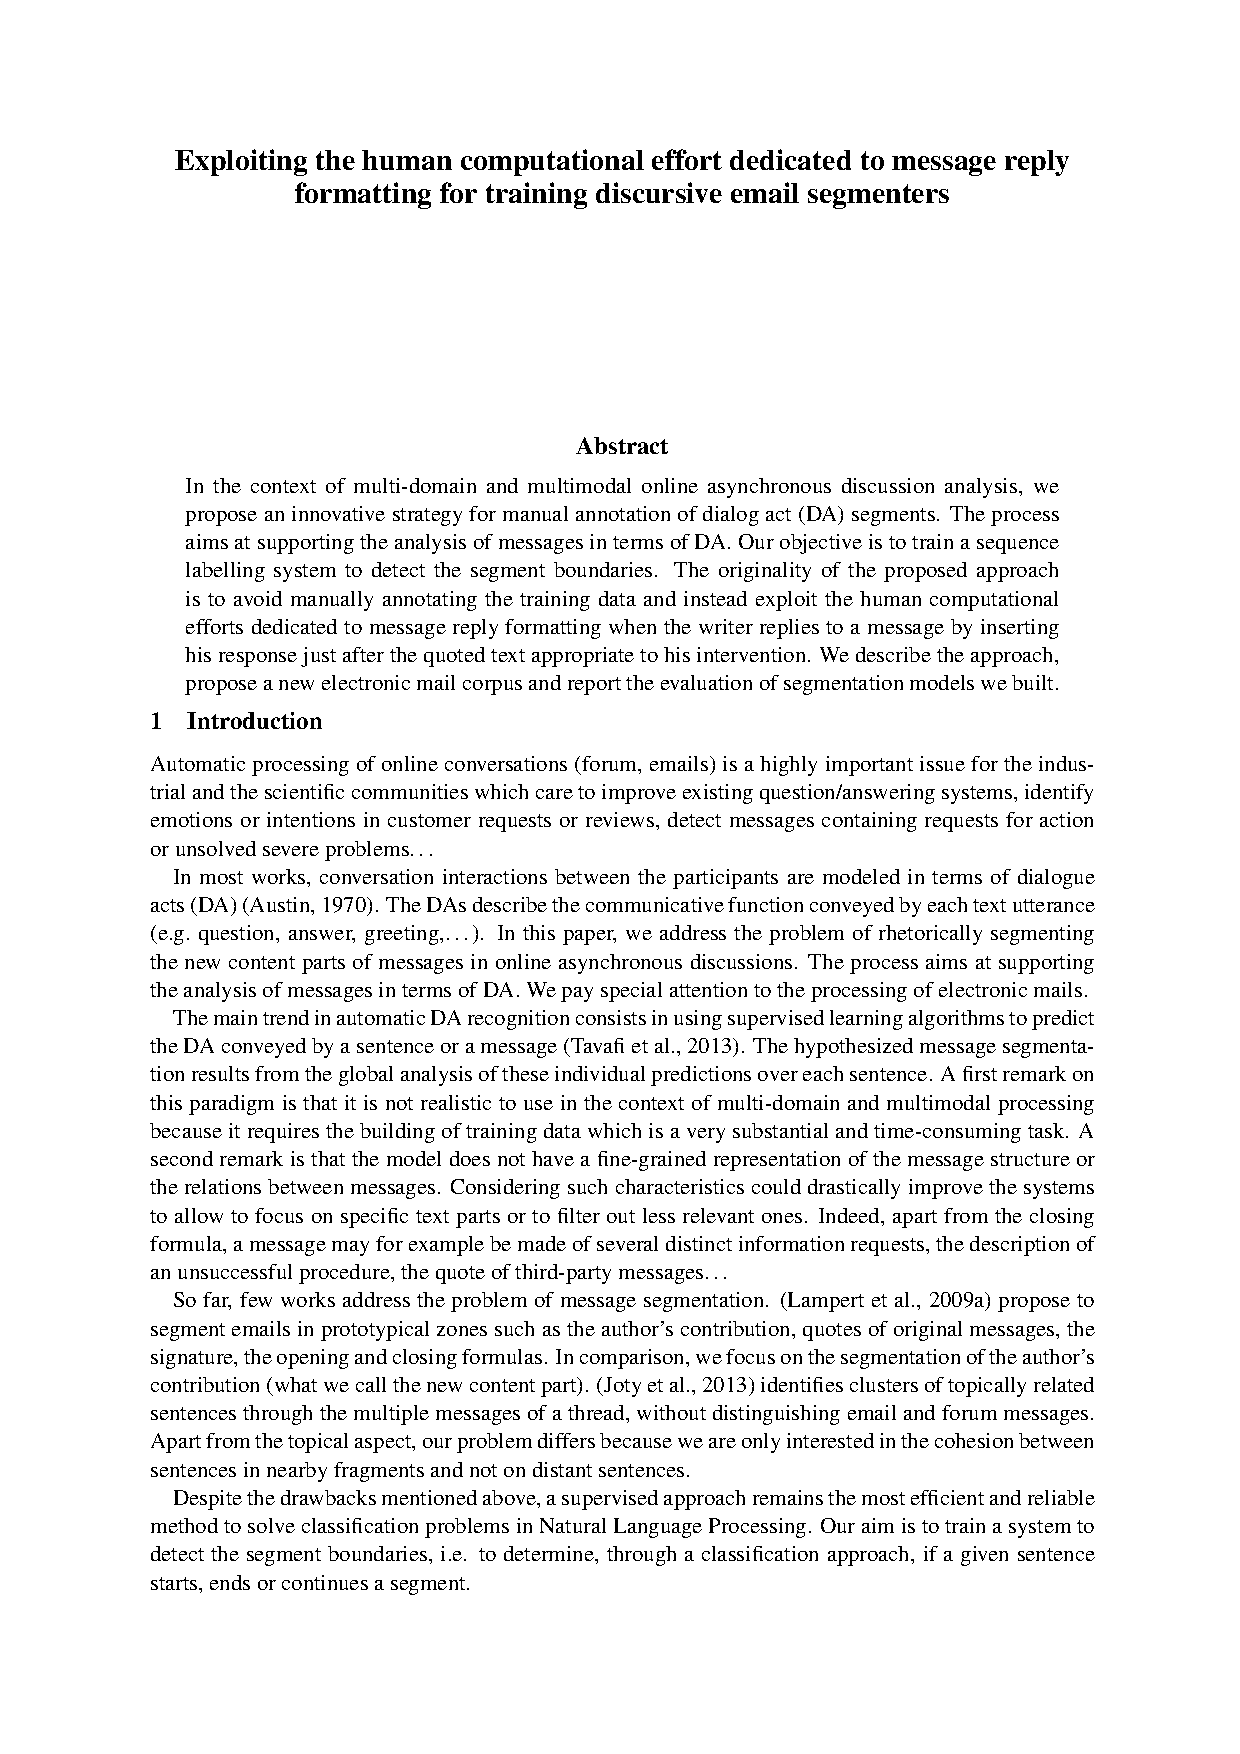
\includepdf[pages=-]{law8.pdf}

\end{appendices}

\addcontentsline{toc}{chapter}{Bibliographie}
\bibliographystyle{authordate2}
\bibliography{bibliography}

\end{document}